\section{The semilocal space $\Gamma\backslash \left(\Q_p\times \Q_q\times \R\right)$}\label{sect3}

Let $S$ be a finite set of places of $\Q$, with $\infty \in S$. We briefly recall the construction of the semilocal adele class space associated to $S$. One replaces the ring of adeles by 
the locally compact ring
$
 \A_{\Q,S}=\prod_{v\in S} \Q_v
$
in which  $\Q$  embeds diagonally. Let
$\cO_{\Q,S}$ be the subring of $\Q$ given by rational numbers whose
denominator only involves primes $p \in S$. In other words,
$
 \cO_{\Q,S}=\{q\in \Q\,|\, |q|_v\leq 1\,,\ \forall v\notin S\}\,.
$
The group $\Gamma$ of invertible elements of  $\cO_{\Q,S}$ is 
\begin{equation}\label{GL1QS}
\Gamma=\GL_1(\cO_{\Q,S})= \{ \pm p_1^{n_1} \cdots p_k^{n_k} \, :\,  p_j
\in S \setminus\{ \infty \} \,,\, n_j\in \Z\}.
\end{equation}
The semilocal adele  class space 
 is the quotient $X_{\Q,S}^{ab}:=\Gamma\backslash\A_{\Q,S}$. The map  
\begin{equation}\label{XQS}
\pi_S:X_{\Q,S}^{ab}\to X_{\Q,S}=\Gamma\backslash\A_{\Q,S}/\left(\prod_{v\in S\setminus \infty}\Z_v^*\right)
\end{equation}
 plays the role of the maximal abelian cover of the  double quotient $X_{\Q,S}$, the semilocal analogue  of $X_\Q$. 
The group 
\begin{equation}\label{JS} J_S=\Gamma\backslash\GL_1(\A_{\Q,S})\simeq \R_+^*\times  \prod_{v\in S\setminus \infty}\Z_v^*
\end{equation}
is the analogue of the idele class group and acts naturally on  $X_{\Q,S}^{ab}$ by multiplication.\newline
We let $p\neq q$ be two primes and  $S=\{ p, q,\infty \}$. The ring $\cO_{\Q,S}$
is $\Z[1/p,1/q]$ and the  abelianized \'etale fundamental group of its spectrum  is 
\begin{equation}\label{pi1}
\pi_1^{e t}(\Spec \, \cO_{\Q,S})^{ab}=\Z_p^*\times \Z_q^*.
\end{equation}
Next we describe the natural stratification of the space $X_{\Q,S}^{ab}$.
\begin{prop}\label{ergodic23} Let $p\neq q$ be two primes,  $S=\{ p, q,\infty \}$ and $\pi_S:X_{\Q,S}^{ab}\to X_{\Q,S}$ as in \eqref{XQS}. Then \newline
$(i)$~The orbits of the action of the group $J_S$ on $X_{\Q,S}^{ab}$ are indexed by the subsets of $S=\{ p, q,\infty \}$ as follows 
$$
\Omega_Z:=\Gamma\backslash\{(a_v)\in \A_{\Q,S}\mid a_v= 0\qqq v \in Z, \ a_v\neq 0\qqq v \notin Z\}\qqq Z\subset S.
$$
$(ii)$~The orbit  $\Omega_{\{p\}}$ associated to the subset $\{p\}\subset S$ is  the inverse image $\pi_S^{-1}(C_p)$ of the periodic orbit  $C_p$ of length $\log p$ (and a similar result holds for the subset $\{q\}\subset S$).\newline
$(iii)$~The orbit $\pi_S^{-1}(C_p)$ is equivariantly isomorphic to the mapping torus of the multiplication by $p$ in the compact group $ \Z_q^*$.	
\end{prop}
\proof $(i)$~Follows from the transitivity of the action of $\GL_1(\Q_v)$ on $\Q_v\setminus \{0\}$ for any  $v$.\newline
$(ii)$~The periodic orbit $C_p$ of length $\log p$  for the action  of the scaling group $\R_+^*$ in $X_{\Q,S}$ is equal to $\pi_S(\Omega_{\{p\}})\subset X_{\Q,S}$ and is identical to the quotient $p^\Z\backslash\R_+^*$. This description shows that $C_p$ appears in the boundary of the free orbit $\pi_S(\Omega_{\emptyset})\subset X_{\Q,S}$ as shown in Figure \ref{fig2}.  \newline
$(iii)$~ One has $\Omega_{\{p\}}=\pi_S^{-1}(C_p)$. The action of $\{\pm q^n\}$ on $\{0\}\times \left(\Q_q\setminus \{0\}\right)\times \R^*$ admits $\{0\}\times \Z_q^*\times \R_+^*$ as fundamental domain. This domain is preserved under the action of $p^\Z$. The quotient 
$$
p^\Z\backslash\left(\Z_q^*\times \R_+^*\right)
$$
is the mapping torus of the multiplication by $p$ in the compact group $ \Z_q^*$.
\endproof
There are $8$ orbits $\Omega_Z$,  $Z\subset S=\{p,q,\infty\}$.  Proposition \ref{ergodic23} describes two of them, the remaining six orbits are described as follows:
\begin{enumerate}
     \item The orbit $\Omega_{\emptyset}\subset X_{\Q,S}^{ab}$  is the idele class group $J_S$ of  \eqref{JS}.
   \item The orbit $\Omega_{\{\infty\}}\subset X_{\Q,S}^{ab}$ is the quotient $\left(\Z_p^*\times \Z_q^*\right)/\pm 1$. 
   \item  The orbit $\Omega_{\{p,q\}}$ is the quotient $(p^\Z q^\Z)\backslash\R_+^*$   \item  The orbit $\Omega_{\{p,\infty\}}$ is the quotient  of $ \Z_q^*/\{\pm 1\}$ by the action of $\Z$ by multiplication by powers of $p$. 
   \item  The orbit $\Omega_{\{q,\infty\}}$ is the quotient  of $ \Z_p^*/\{\pm 1\}$ by the action of $\Z$ by multiplication by powers of $q$. 
   \item The orbit  $\Omega_{\{p,q,\infty\}}$ is a single point.
\end{enumerate}
To be more precise one can describe for each orbit the corresponding $C^*$-algebra up to Morita equivalence. For $(3)$ one obtains the noncommutative torus associated to the irrational number $\log p /\log q$. For $(4)$ one gets the cross product  $
C(\Z_q^*/\pm 1)\ltimes p^\Z
$
and similarly for $(5)$. Finally for $(6)$ one gets the group ring $C^*(\Gamma)$. By construction the group $J_S$ acts by automorphisms on these $C^*$-algebras.
\vspace{-.2in}

\begin{figure}[H]
    \centering\vspace*{.3in}
    
\subfloat[]{{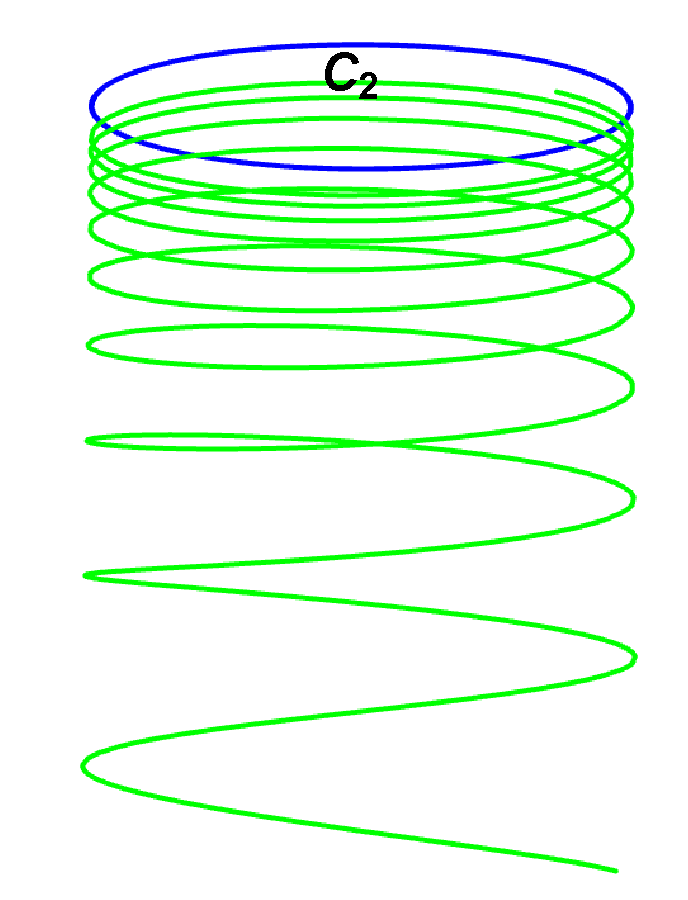
\includegraphics[width=4cm,valign=m]{wirling1.pdf} }}%
    \hspace{1in}
\subfloat[]{{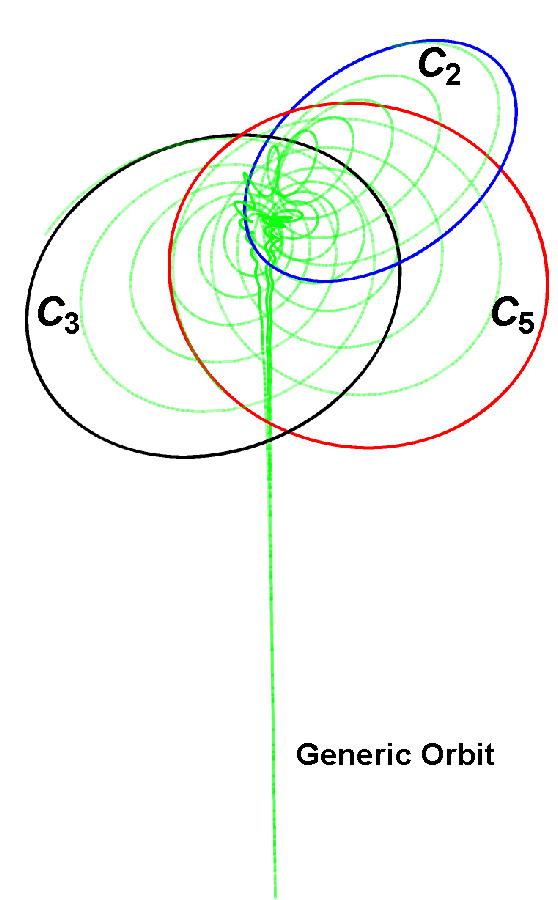
\includegraphics[width=5.5cm,,valign=m]{flowers.pdf} }}%
    \caption{(A) shows how the generic orbit (in green) for the action of $\R_+^*$ on $X_\Q$ is dense in the periodic orbit $C_p$. This holds for any $p$. (B) shows how the density of the generic orbit in every $C_p$ imitates the density of the generic point of $\Spec\,\Z$ (compare  with \cite{Manin}, page 16).}%
    \label{fig2}%
\end{figure}


\subsection*{Proof of Theorem \ref{mainintro}}
This follows from Proposition \ref{ergodic23} $(iii)$, together with the following facts :
\begin{itemize}
\item The abelianized \'etale fundamental group $\pi_1^{e t}(\Spec \, \Z[1/q])^{ab}$  is canonically isomorphic to $\Z_q^*$.
\item The image $\pi_1^{e t}(r^*)\left\{F r o b_{p}\right\}$ is equal to $p\in  \Z_q^*$.
\end{itemize}
As in the proof of Theorem \ref{mainglobalintro}, the first fact follows using \cite{Lenstra} (Corollary 6.17), together with the determination of the maximal abelian extension of $\Q$ only ramified at $q$ (obtained by adjoining all roots of unity of order a power of $q$). Its Galois group is $\Z_q^*$. The second fact follows since the action of $\left\{F r o b_{p}\right\}$ on roots of unity is given by raising to the power $p$.
